
\section{Trénovacia databáza zbraní}
\label{sec:databaza}
Pre správne trénovanie klasifikátorov a neurónových sietí je dôležité mať dáta v dostatočnom počte a správne označené.
Trénovacia databáza je získaná z niekoľkých zdrojov.
\begin{enumerate}
    \item[$\bullet$] \textbf{IMFDB}\footnote{\url{http://www.imfdb.org/wiki/Main_Page}} - je databáza záberov z filmov, v ktorých sa nachádzajú zbrane.
    Obsahuje nie len celkové scény, ale aj samostatné obrázky zbraní, ktoré sa v danej scéne nachádzajú.
    Pre túto prácu je potrebné, aby daný obrázok obsahoval iba zbraň, preto je potrebné obrázky z tejto databázy ručne odfiltrovať na samotné zbrane a scény so zbraňami.
    Následne ich potom zaradiť do správnej kategórie na krátke a dlhé.
    \item[$\bullet$] \textbf{ImageNet}\footnote{\url{http://www.image-net.org/}} - je databáza obrázkov, ktorá obsahuje viac ako 14 miliónov obrázkov vo viac ako 21000 kategóriách.
    Výhodou tejto databázy je, že obrázky už patria do určenej kategórie a tak nie je potrebné ich ručne prechádzať a kategorizovať.
    \item[$\bullet$] \textbf{Google}\footnote{\url{http://www.google.com}} - pre doplnenie a zväčšenie počtu obrázkov je možné použiť google vyhľadávanie.
    Tak ako v prípade IMFDB bude potrebné obrázky ručne kategorizovať.
    \item[$\bullet$] \textbf{Free3D}\footnote{\url{https://free3d.com/3d-models/weapons}} - databáza voľne dostupných 3D modelov zbraní s textúrami v rôznych formátoch.
\end{enumerate}

Databáza zbraní z prvých 3 zdrojov je možné použiť na klasficikáciu zbraní do 2 kategórií na krátke a dlhé zbrane.
Pre trénovanie neurónových sietí na určenie náklonu zbrane v obraze bude potrebné použiť 3D modely zbraní a následne pomocou nich vygenerovať
    obrázky zbraní v požadovaných natočeniach zbrane v obraze.

\subsection{Generovanie dát z 3D modelov}
\label{subsec:generovanie3d}
Generovanie obrázkov pre určenie náklonu zbrane v scéne bude prebiehať pomocou databázy 3D modelov zo zdroja Free3D.
Následne sa použije software SYDAGenerator\footnote{\url{http://www.fit.vutbr.cz/~igoldmann/app/SYDAGenerator}} na generovanie obrázkov z 3D modelov,
    do ktorého je potrebné vložiť 3D model vo formáte g3db a pozadie scény.

Keďže 3D modely, ktoré budú použité nie sú v požadovanom formáte, je potrebné ich prekonvertovať, to je možné urobiť
    pomocou nástroja \textbf{fbx-conv}\footnote{\url{https://github.com/libgdx/fbx-conv}}.
Tento nástroj podporuje konvertovanie 3D modelov z formátu \textit{fbx}, alebo \textit{obj} do požadovaného formátu \texttt{g3db}.

\subsection{Augmentácia obrázkov}
\label{subsec:augmentacia}
Ako bolo opísané v kapitole \ref{sec:preprocessing} jedna z možností zväčšenia počtu vstupných dát a zlepšenia generalizácie pri klasifikácii je augmentácia vstupných dát.
V tejto práci môžeme rozdeliť augmentáciu dát do dvoch skupín, prvý druh augmentácie bude prebiehať pre trénovanie klasifikátorov, ktoré
    určujú typ zbrane, druhý druh augmentácie bude prebiehať pri obrázkoch určených pre náklon zbrane.

Pri augmentácií dát pre klasifikovanie dvoch tried, na krátke a dlhé zbrane, prebehne niekoľko transfomácií obrázka.
\begin{enumerate}
    %\item[$\bullet$] \textbf{priblíženie} - priblíženie alebo oddialenie vstupného obrázka
    \item[$\bullet$] \textbf{Rotácia} - obrázky budú rotované o náhodný uhol v rozmedzí 0-180 stupňov.
    \item[$\bullet$] \textbf{Preklopenie} - vertikálne alebo horizonálne preklopenie obrázka.
    \item[$\bullet$] \textbf{Posun} - posun obrázka po x-ovej a y-ovej osi.
    \item[$\bullet$] \textbf{Výplň} - pri rotácií alebo posune obrázka môže vzniknúť čierna plocha pixelov, tieto čierne pixely je potrebné vyplniť.
    Tieto čierne pixely budú doplnené hraničným pixelom obrázka, ktorý bude nakopírovaný až po nový okraj.
\end{enumerate}

\begin{figure}[H]
    \centering
    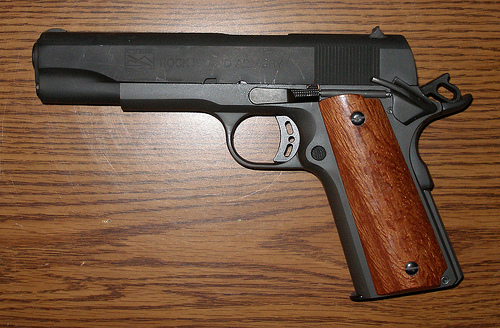
\includegraphics[width=0.4\textwidth]{weapons/weapon}
    \qquad
    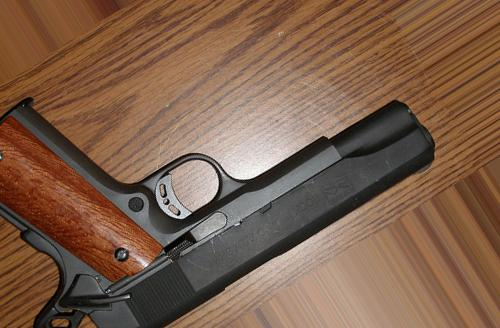
\includegraphics[width=0.4\textwidth]{weapons/weapon-augmented}
    \caption{Pôvodny obrázok (vľavo), augmentovaný obrázok (vpravo)}
    \label{pic:imageAugmented}
\end{figure}

Druhý typ augmentácie dát prebieha pri obrázkoch, ktoré boli vygenerované pomocou 3D modelu.
Keďže nie je potrebné generovať všetky polohy otočenia od 0 po 360 stupňov, stačí vygenerovať dáta v polohách od 0 po 90 stupňov a od 270 do 359 stupňov.
Zvyšné polohy je možné dogenerovať pomocou transformácie obrázka, pomocou vertikálneho alebo hotizontálneho preklopenia.
Avšak v tomto prípade je potrebné po transformácii obrázka vyrátať novú hodnotu uhla transformovaného obrázka, to je možné dosiahnuť pomocou niekoľkých
    jednoduchých vzorcov.

\textbf{Roll}, pri natočení modelu v ose roll, je potrebné aplikovať horizontálne preklopenie obrázka.
Následne uhol transformovaného obrázka $trans\_angle$ bude vypočítaný z pôvodného uhla $angle$.
V rozsahu $270 \leq angle \leq 359$ podľa:
\begin{equation}
    trans\_angle = -angle + 540 
\end{equation}
a v rozsahu $0 \leq angle \leq 90$ podľa:
\begin{equation}
    trans\_angle = abs(angle - 180)
\end{equation}

\begin{figure}[H]
    \centering
    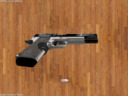
\includegraphics[width=0.3\textwidth]{weapons/roll_300}
    \quad
    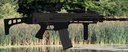
\includegraphics[width=0.3\textwidth]{weapons/roll_0}
    \quad
    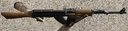
\includegraphics[width=0.3\textwidth]{weapons/roll_70}
    \caption{Natočenie zbrane v ose roll, 300 stupňov(vľavo), 0 stupňov(v strede), 70 stupňov(vpravo)}
    \label{pic:rollrotation}
\end{figure}

\textbf{Yaw}, pri natočení v ose yaw, sa aplikuje vertikálne preklopenia obrázka.
Uhol transformovaného obrázka sa vypočíta v rozsahu $270 \leq angle \leq 359$ podľa:
\begin{equation}
    trans\_angle = abs(angle - 540)
\end{equation}
a v rozsahu $0 \leq angle \leq 90$ podľa:
\begin{equation}
    trans\_angle = abs(angle - 180)
\end{equation}

\begin{figure}[H]
    \centering
    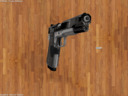
\includegraphics[width=0.3\textwidth]{weapons/yaw_300}
    \quad
    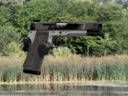
\includegraphics[width=0.3\textwidth]{weapons/yaw_0}
    \quad
    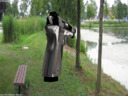
\includegraphics[width=0.3\textwidth]{weapons/yaw_75}
    \caption{Natočenie zbrane v ose yaw, 300 stupňov(vľavo), 0 stupňov(v strede), 75 stupňov(vpravo)}
    \label{pic:yawrotation}
\end{figure}

\textbf{Pitch}, v ose pitch postačuje vygenerovať obrázok zbrane s náklonom 0 stupňov so smerovaním hlavne zbrane doprava.
Počas augmentácie dát sa môže aplikovať horizontálne preklopenie a následne sa tento vstupný obrázok otočí o náhodný uhol.
Preto nie je potrebný žiaden další prepočet uhla.

\begin{figure}[H]
    \centering
    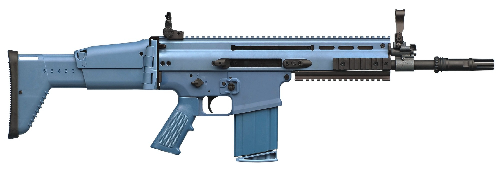
\includegraphics[width=0.3\textwidth]{weapons/pitch_0}
    \quad
    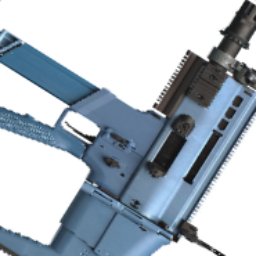
\includegraphics[width=0.2\textwidth]{weapons/pitch_60}
    \quad
    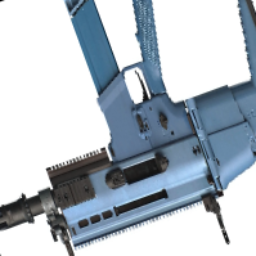
\includegraphics[width=0.2\textwidth]{weapons/pitch_200}
    \caption{Natočenie zbrane v ose pitch, 0 stupňov(vľavo), 60 stupňov(v strede), 200 stupňov(vpravo)}
    \label{pic:yawrotation}
\end{figure}
